\chapter{Conclusion and Future Directions}
\label{chap:chap8}
%
This thesis contributes to the development of computer vision and pattern recognition techniques for image compression and image classification applications. A summary of the contributions of this thesis are shown in Fig.~\ref{fig: Thesis_work}. This thesis makes three significant contributions: (i) incoherent and robust sensing matrix, (ii) locality-aware projection matrix, and (iii) twin relaxed projection matrix for regression-based image classification.

First, we presented a novel algorithm to develop an incoherent and robust sensing matrix for CS-based image compression model. In CS-based systems, recovery performance largely depends on the sensing matrix and its characteristics, such as incoherence and tightness, which helps in extracting fewer yet significant measurements. However, the underlying data (images) represented using a sparsifying basis suffers from sparse encoding error as explained in Section~\ref{sec: Chap_1_intro_CS}. In real-world applications, images are not precisely sparse but compressible, which requires careful sensing matrix design; otherwise, the error matrix would be amplified when projected onto the measurement domain. The proposed IR-PMD algorithm designs the sensing matrix for image compression to reduce the frame's pairwise correlation and tightness by restricting eigenvalues. Further, the proposed method incorporates an $\ell_{2,1}$-norm based regularization term to reduce the impact of outliers and noisy data.
%
\begin{figure}
   \centering
   \scalebox{.7}{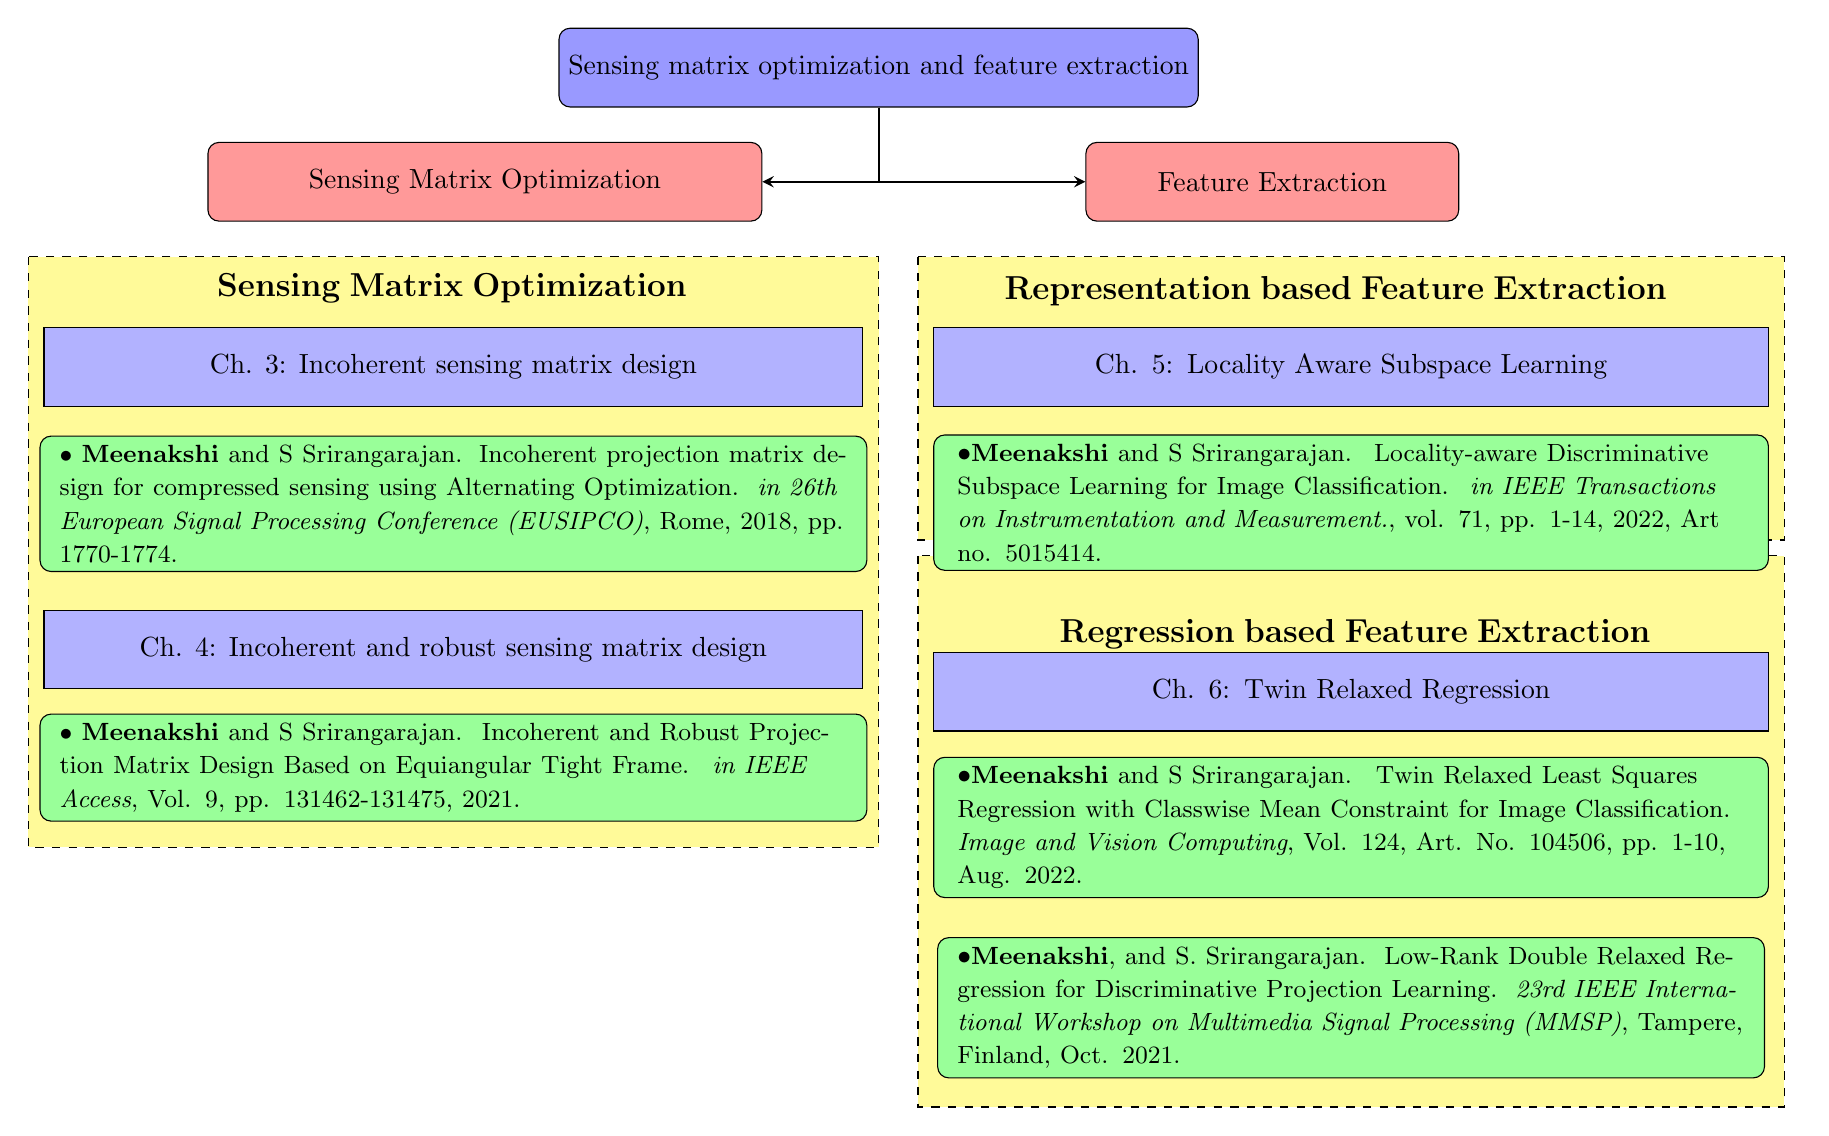
\begin{tikzpicture}
\usetikzlibrary{shapes.geometric, arrows}
\draw  [dashed, fill=yellow!40] (-10.8,-2.4) rectangle (0.00,-9.9);

\draw  [dashed, fill=yellow!40]   (0.5,-2.4) rectangle (11.5,-6);

\draw  [dashed, fill=yellow!40]   (0.50,-6.2) rectangle (11.5,-13.2);

\tikzstyle{L1} = [rectangle, rounded corners, minimum width=3cm, minimum height=1cm,text centered, draw=black, fill=green!40]

\tikzstyle{L2a} = [rectangle, minimum width=10.4cm, minimum height=1cm,text centered, draw=black, fill=blue!30]



\tikzstyle{L2d} = [rectangle, text width=10cm, minimum width=10.6cm, minimum height=1cm,text centered, draw=black, fill=blue!30]

\tikzstyle{L3a} = [rectangle,rounded corners, text width=9.5cm,  minimum width=10cm, minimum height=1cm,draw=black, fill=green!40]

\tikzstyle{L3a1} = [rectangle,rounded corners, text width=10cm,  minimum width=10.6cm, minimum height=1cm,draw=black, fill=green!40]


\tikzstyle{L3b} = [rectangle,rounded corners, text width=10cm,  minimum width=10.5cm, minimum height=1cm,draw=black, fill= green!40]

\tikzstyle{L3c} = [rectangle,rounded corners, text width=10cm,  minimum width=10.5cm, minimum height=1cm,draw=black, fill= green!40]

\tikzstyle{L4} = [rectangle,rounded corners, text width=6.5cm,  minimum width=6cm, minimum height=1cm,draw=black, fill=cyan!15]

\tikzstyle{arrow} = [thick,->,>=stealth]

\node (a1) [L1,fill=blue!40] {Sensing matrix optimization and feature extraction};

\node (a2) [L1, text width=6.8cm, below of=a1, yshift=-.45cm, xshift=-5cm,fill=red!40] {Sensing Matrix Optimization};

\node (a3) [L1,text width=4.5cm, below of=a1, yshift=-.45cm, xshift=5cm,fill=red!40] {Feature Extraction};

\draw [arrow] (a1) |- (a2);
\draw [arrow] (a1) |- (a3);

\node (a4) [L2a, below of=a1, yshift=-2.8cm, xshift=-5.4cm] {Ch. 3: Incoherent sensing matrix design};
\node (a5) [L3b, below of=a4,yshift=-.74cm] {\small{\textbf{$\bullet$ Meenakshi} and S~Srirangarajan.
\newblock Incoherent projection matrix design for compressed sensing using Alternating Optimization.
\newblock {\em in 26th European Signal Processing Conference (EUSIPCO)}, Rome, 2018, pp. 1770-1774.}};


\node (a6) [L2a, below of=a5,yshift=-.85cm] {Ch. 4: Incoherent and robust sensing matrix design};
\node (a7) [L3c, below of=a6,yshift=-.50cm]{\small{\textbf{$\bullet$ Meenakshi} and S~Srirangarajan.
\newblock Incoherent and Robust Projection Matrix Design Based on Equiangular Tight Frame.
 \newblock {\em in IEEE Access}, Vol. 9, pp. 131462-131475, 2021.} };
\node (a15) [L2d, below of=a1, yshift=-2.8cm,xshift=6cm] {Ch. 5: Locality Aware Subspace Learning };
\node (a16) [L3a1, below of=a15,yshift=-0.725cm]  {$\bullet$\small{\textbf{Meenakshi} and S~Srirangarajan.
\newblock Locality-aware Discriminative Subspace Learning for Image Classification.
\newblock {\em in IEEE Transactions on Instrumentation and Measurement.}, vol. 71, pp. 1-14, 2022, Art no. 5015414.}};

\node (a17) [L2d, below of=a16,yshift=-1.4cm] {Ch. 6: Twin Relaxed Regression };
\node (a18) [L3a1, below of=a17, yshift=-0.725cm]  {$\bullet$\small{\textbf{Meenakshi} and S~Srirangarajan.
\newblock Twin Relaxed Least Squares Regression with Classwise Mean Constraint for Image Classification.
\newblock{ \em Image and Vision Computing}, Vol. 124, Art. No. 104506, pp. 1-10, Aug. 2022.}};

\node (a19) [L3c, below of=a18, yshift=-1.29cm]  {$\bullet$\small{\textbf{Meenakshi}, and S. Srirangarajan.
\newblock Low-Rank Double Relaxed Regression for Discriminative Projection Learning.
\newblock {\em 23rd IEEE International Workshop on Multimedia Signal Processing (MMSP)}, Tampere, Finland, Oct. 2021.}}; 
\node[text width=7cm,thick] at (-4.9,-2.8) {\large{\textbf{Sensing Matrix Optimization}}};
\node[text width=10cm,thick] at (6.6,-2.84) {\large{\textbf{Representation based Feature Extraction}}};
\node[text width=9cm,thick] at (6.8,-7.20) {\large{\textbf{Regression based Feature Extraction}}};


\end{tikzpicture}

}
 \caption{Summary of the research contributions and publications from this thesis.}
    \label{fig: Thesis_work}
\end{figure}
%
The proposed approach first constructs an equiangular tight frame by restricting the eigenvalues of the desired Gram matrix. Next, an incoherent sensing matrix is obtained from the equiangular tight frame considering sparse encoding error for robustness. Additionally, an $\ell_{2,1}$-norm is used as a compromise between $\ell_{0}$-norm and $\ell_{1}$-norm, as it is more robust than the Frobenius norm, and it promotes row-sparsity. An adaptive weight with the fidelity term helps minimize the sensing matrix energy. The experimental results on synthetic and real data sets validate the superiority of the proposed robust sensing matrix design. Although, the proposed approach optimizes the sensing matrix while preserving the incoherence and tightness of frame, it does not provide a closed form solution. In addition, the proposed approach does not have a strong convergence proof, although, we provide an alternating minimization based algorithm with empirical convergence.

In the next part of the thesis, we addressed the design of a projection matrix for extracting a set of significant features from high-dimensional data. We observed that data plays a vital role, however, it results in large memory and computational requirements in real-life applications. In addition, large data sets result in many challenges (refer Section~\ref{sec: Chap_1_feature Extraction overview}) and require the learning models to handle large amounts of data. A large number of features leads to a large, high-dimensional feature matrix, increasing the computational and storage requirements. Hence, for representation-based feature extraction, we extract key features from raw data to uncover the underlying structure for the learning algorithms. Additionally, we exploit the adaptive local structure of the data in terms of the neighborhood relationship among the data samples. Furthermore, the proposed approach introduces a new transition matrix to seamlessly integrate subspace learning with regression and exploits the low-rank structure of the self-representation matrix. Results of the experimental analysis on public data sets validate the ability of our proposed method to correctly and efficiently learn the salient features, especially with small training numbers.

In the final part of this thesis, we presented a regression-based feature extraction for image classification. We introduced a twin matrix with a relaxed target to preserve the underlying structure of the data while expanding the inter-class margins. The relaxed target matrix and a twin matrix in TRLSR allow greater flexibility in learning the projections. Additionally, a classwise mean constraint is introduced to retain the data's intra-class similarity, which is beneficial in learning more discriminative projections. An $\ell_{2,1}$-norm-based regularization on the optimized projections is incorporated to extract more significant features, and limit the impact of noise and overfitting. The results for image classification on public data sets validate the efficiency of the proposed algorithm compared to the state-of-the-art algorithms. A limitation of the feature extraction methods, presented in Chapters~\ref{chap:chap5} and~\ref{chap:chap6}, is that their mathematical formulations are non-convex. We solve these using ADMM-style algorithm and have only provided a weak convergence. However, the convergence curves in Fig.~\ref{fig: AR_PIE_conv} and Fig.~\ref{Fig: TRLSR_Data_conv} show fluctuations when the number of iterations are large. This indicates that ADMM cannot guarantee that the objective function values of TRLSR and LADSL methods would converge when there are more than two variables. In practice, such conditions are quite probable. Thus, a convex relaxation of these objective functions is one of the possible future research directions.
%
\section{Future Directions}
\label{sec: Future_work}
%
In this section, we discuss the possible future research directions based on this thesis. In the proposed algorithms, we employ several weight parameters that determine the contribution of each of the terms in the objective function. Setting appropriate values for these weight parameters is an important task. It would be good to develop a systematic approach to choose the weight parameters to achieve an optimal solution and reduce the number of iterations. In Chapter~\ref{chap:chap5} and Chapter~\ref{chap:chap6}, we have explored the design of projection matrix for dimensionality reduction by exploiting the $\ell_{2,1}$-norm for row-sparsity and robustness. In the future, a different regularizer norm such as ($\ell_{1} - \ell_{2}$)-norm and $\text{det}-\ell_{2,1}$-norm can be used to extend the work. The methods discussed in this thesis, optimize the projection matrix to transform high-dimensional data to the binary label space. The methods presented focus on the projection matrix by exploiting the self-representation property of the data. The work can be extended to joint dictionary and projection matrix learning to utilize the sparse representation of the underlying data using overcomplete dictionaries. Furthermore, the work can be extended by using CNNs to efficiently apply the learning algorithms on large-scale data sets. Lastly, the work can be extended to represent training data as a third-order tensor, instead of vectorizing it for optimization, to improve the joint dimensionality reduction and feature extraction framework.